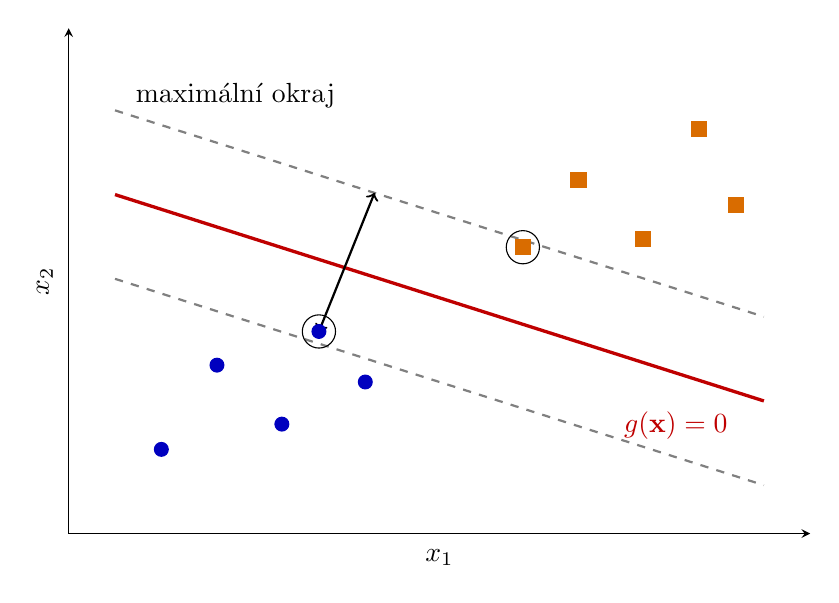
\begin{tikzpicture}
    \begin{axis}[
        width=11cm,height=8cm,
        xmin=0,xmax=8,ymin=0,ymax=6,
        axis lines=left,xlabel={$x_1$},ylabel={$x_2$},
        xtick=\empty,ytick=\empty,
        label style={font=\normalsize},
        every node/.style={font=\normalsize},
        clip=false
    ]
        \addplot[only marks,mark=*,mark size=2.5pt,blue!75!black]
            coordinates{(1,1)(1.6,2)(2.3,1.3)(2.7,2.4)(3.2,1.8)};
        \addplot[only marks,mark=square*,mark size=2.7pt,orange!85!black]
            coordinates{(4.9,3.4)(5.5,4.2)(6.2,3.5)(6.8,4.8)(7.2,3.9)};
        \addplot[red!75!black,very thick,domain=0.5:7.5]{-0.35*x+4.2};
        \addplot[gray,dashed,thick,domain=0.5:7.5]{-0.35*x+3.2};
        \addplot[gray,dashed,thick,domain=0.5:7.5]{-0.35*x+5.2};
        \addplot[only marks,mark=o,mark size=6pt,black]
            coordinates{(2.7,2.4)(4.9,3.4)};
        \node[red!75!black] at (axis cs:6.55,1.28){\(g(\mathbf{x})=0\)};
        \node at (axis cs:1.8,5.2){maximální okraj};
        \draw[<->,thick] (axis cs:2.7,2.4)--(axis cs:3.3,4.045);
    \end{axis}
\end{tikzpicture}
